\chapter{Assessing the stability}

The results of the previous chapter highlighted not only the impact of the parameters on the clustering output, but also raised the question of interpretation stability. While there are parameters which are designed to affect the clustering output, such as the resolution parameter, the community detection, the objective function or the feature space, there are some factors that should not be responsible for obtaining different results.

One if these factors is the random seed. It is not an expected behaviour to get different partitions and different downstream biological interpretations if only the seed is changed.

\section{ClustAssess}
Under the supervision of professor Irina Mohorianu and Arash Shahsavari, I was part of the team that developed the R package \verb|ClustAssess| \footnote{GitHub official repository: \url{https://github.com/Core-Bioinformatics/ClustAssess}} \cite{clustassess}.

The package has several functionalities, including:
\begin{itemize}
    \item determine the optimal number of clusters using PAC (method based on cumulative distribution)
    \item calculate the Element-Centric Similarity (ECS) between two flat, overlapping or hierarchical partitions
    \item calculate the Element-Centric Consistency (ECC) of a list containing flat, overlapping and hierarchical partitions
    \item calculate the marker gene similarity across each cell
    \item stability-based parameter assessment pipeline.
\end{itemize}
This chapter will contain a description of the package components that I contributed on research and developing, namely calculating the ECS score and creating the stability pipeline.

\section{ECS calculation}
As far as we are concerned, the Python package \verb|CluSim| \footnote{GitHub official repository: \url{https://github.com/Hoosier-Clusters/clusim}} \cite{Gates2019b}, which is developed and maintained by the authors of the ECS paper \cite{Gates2019}, is the only official source that contains an implementation of the Element-Centric Similarity measure.


The ClustAssess package offers an R implementation of this score. The implementation follows the steps presented in the article presented above. For each partition, the cluster affiliation graph is determined, followed by calculating the cluster-induced element graph and teh affinity matrix. Once the affinity matrices are calculated, the ECS can be calculated as the L1 distance between them.

\subsection{Optimising the calculation of the ECS}
However, as stated in the first chapter, computing the PPR matrix for flat disjoint partitions can be done using the formula \ref{eq:affinity-disjoin}. As it can be observed, for each pair of points, there can only be three values, all of them being independent on the nature of the points. We will use this observation to prove that the calculation of the ECS score can be optimised.



Let $\mathcal{A}$ and $\mathcal{B}$ be two partitions of the same set of points $\mathcal{P}$. Let $C_a^\mathcal{A}$ denote the $\text{a}^{th}$ cluster of the partition $\mathcal{A}$, and $C_b^\mathcal{B}$ denote the $\text{b}^{th}$ cluster of the partition $\mathcal{B}$. Denote the length of the clusters as follows: $|C_a^{\mathcal{A}}| = c_a \text{ and } |C_b^{\mathcal{B}}| = c_b$.

\begin{remark} \label{remark:pii}
    $p_{ii}^\mathcal{A} - p_{ii}^\mathcal{B} = p_{ij}^\mathcal{A} - p_{ij}^\mathcal{B}$, for any $i, j \in C_a^\mathcal{A} \cap C_b^\mathcal{B}$
\end{remark}

\begin{proof}
    The proof is immediate when $i = j$.

    For $i \neq j$, from the Equation \ref{eq:affinity-disjoin}, we will have:
    $ 
        \displaystyle
        \begin{cases}
            p_{ij}^\mathcal{A} &= \frac{\alpha}{c_a} \\
            p_{ij}^\mathcal{B} &= \frac{\alpha}{c_b} 
        \end{cases}
    $.
    Therefore, 
    \begin{equation} \label{eq:rem1-i}
        p_{ij}^\mathcal{A} - p_{ij}^\mathcal{B} = \alpha\left(\frac{1}{c_a} - \frac{1}{c_b}\right) 
    \end{equation}

    From the same equation, we get that 
    $ 
        \displaystyle
        \begin{cases}
            p_{ii}^\mathcal{A} &= 1-\alpha + \frac{\alpha}{c_a} \\
            p_{ii}^\mathcal{B} &= 1-\alpha + \frac{\alpha}{c_b} 
        \end{cases}
    $. Therefore, 
    \begin{equation} \label{eq:rem1-ii}
        p_{ii}^\mathcal{A} - p_{ii}^\mathcal{B} = \left(1-\alpha + \frac{\alpha}{c_a}\right) - \left(1-\alpha+\frac{\alpha}{c_b}\right) = \alpha\left(\frac{1}{c_a}-\frac{1}{c_b}\right)
    \end{equation}

    From \ref{eq:rem1-i} and \ref{eq:rem1-ii}, we get that $p_{ii}^\mathcal{A} - p_{ii}^\mathcal{B} = p_{ij}^\mathcal{A} - p_{ij}^\mathcal{B}$.
\end{proof}

\begin{remark} \label{remark:ecs-constant}
    $\displaystyle\mathcal{S}_i(\mathcal{A}, \mathcal{B}) = 1-\frac{1}{2}\left(|C_a^\mathcal{A} \cap C_b^\mathcal{B}|\cdot \left|\frac{1}{c_a} - \frac{1}{c_b}\right| + |C_a^\mathcal{A} \cap (\mathcal{P} \setminus C_b^{\mathcal{B}})| \cdot \frac{1}{c_a} + |(\mathcal{P} \setminus C_a^\mathcal{A}) \cap C_b^\mathcal{B}|\cdot \frac{1}{c_b} \right)$, for any $i \in C_a^\mathcal{A} \cap C_b^\mathcal{B}$.
\end{remark}

\begin{proof}
   In order to calculate the Element-Centric Similarity between partitions $\mathcal{A}$ and $\mathcal{B}$ in the point $i$, we must use the formula as described in the Equation \ref{eq:def-ecs}.

   To define $p_{ij}^{\mathcal{A}}$ and $p_{ij}^{\mathcal{B}}$, we must explore all four cases of labeling the point $j$. 
    
   \textbf{Case 1:} $j \in C_a^{\mathcal{A}} \cap C_b^{\mathcal{B}}$ ($j$ belongs to the same cluster as $i$ in both partitions.)

   Using the formula from \ref{eq:affinity-disjoin}, we have $\displaystyle
    \begin{cases}
        p_{ij}^\mathcal{A} &= \frac{\alpha}{c_a} \\
        p_{ij}^\mathcal{B} &= \frac{\alpha}{c_b} 
    \end{cases}$. Therefore, 
    \[ p_{ij}^\mathcal{A} - p_{ij}^\mathcal{B} = \alpha \left(\frac{1}{c_a} - \frac{1}{c_b}\right) .\]

    This equation also holds when $j = i$, as proven in Remark \ref{remark:pii}.

    \textbf{Case 2:} $j \in C_a^\mathcal{A} \cap (\mathcal{P} \setminus C_b^{\mathcal{B}})$ ($j$ belongs to the same cluster as $i$ only in the first partition.)

   Using the formula from \ref{eq:affinity-disjoin}, we have $\displaystyle
    \begin{cases}
        p_{ij}^\mathcal{A} &= \frac{\alpha}{c_a} \\
        p_{ij}^\mathcal{B} &= 0
    \end{cases}$. Therefore, 
    \[ p_{ij}^\mathcal{A} - p_{ij}^\mathcal{B} = \alpha \frac{1}{c_a} .\]

    \textbf{Case 3:} $j \in (\mathcal{P} \setminus C_a^\mathcal{A}) \cap  C_b^{\mathcal{B}}$ ($j$ belongs to the same cluster as $i$ only in the second partition.)

   Using the formula from \ref{eq:affinity-disjoin}, we have $\displaystyle
    \begin{cases}
        p_{ij}^\mathcal{A} &= 0 \\
        p_{ij}^\mathcal{B} &=\frac{\alpha}{c_b}
    \end{cases}$. Therefore, 
    \[ p_{ij}^\mathcal{A} - p_{ij}^\mathcal{B} = \alpha \frac{1}{c_b} .\]

    \textbf{Case 4:} $j \in (\mathcal{P} \setminus C_a^\mathcal{A}) \cap  (\mathcal{P} \setminus C_b^{\mathcal{B}})$ ($j$ belongs to a different cluster than $i$ both partitions.)

   Using the formula from \ref{eq:affinity-disjoin}, we have $\displaystyle
    \begin{cases}
        p_{ij}^\mathcal{A} &= 0 \\
        p_{ij}^\mathcal{B} &=0
    \end{cases}$. Therefore, 
    \[ p_{ij}^\mathcal{A} - p_{ij}^\mathcal{B} = 0 .\]


    These four cases are exhaustive so $\displaystyle \sum_{j = 1}^N |p_{ij}^{\mathcal{A}} - p_{ij}^{\mathcal{B}} |$ will be equivalent to % according to \ref{eq:def-ecs}, $\mathcal{S}_i(\mathcal{A}, \mathcal{B})$ will be:

    \[
        \begin{aligned}
            &\sum_{j \in C_a^{\mathcal{A}} \cap C_b^{\mathcal{B}}} |p_{ij}^{\mathcal{A}} - p_{ij}^{\mathcal{B}} | + \sum_{j \in C_a^\mathcal{A} \cap (\mathcal{P} \setminus C_b^{\mathcal{B}})} |p_{ij}^{\mathcal{A}} - p_{ij}^{\mathcal{B}} | + \sum_{j \in (\mathcal{P} \setminus C_a^\mathcal{A}) \cap  C_b^{\mathcal{B}}} |p_{ij}^{\mathcal{A}} - p_{ij}^{\mathcal{B}} | + \sum_{j \in (\mathcal{P} \setminus C_a^\mathcal{A}) \cap  (\mathcal{P} \setminus C_b^{\mathcal{B}})} |p_{ij}^{\mathcal{A}} - p_{ij}^{\mathcal{B}} | = \\
            %
            = &\sum_{j \in C_a^{\mathcal{A}} \cap C_b^{\mathcal{B}}} \left|\alpha\left(\frac{1}{c_a} - \frac{1}{c_b}\right)\right| + \sum_{j \in C_a^\mathcal{A} \cap (\mathcal{P} \setminus C_b^{\mathcal{B}})} \left|\alpha\frac{1}{c_a}\right| + \sum_{j \in (\mathcal{P} \setminus C_a^\mathcal{A}) \cap  C_b^{\mathcal{B}}} \left|\alpha\frac{1}{c_b}\right| + \sum_{j \in (\mathcal{P} \setminus C_a^\mathcal{A}) \cap  (\mathcal{P} \setminus C_b^{\mathcal{B}}} |0 | = \\
            %
            = &\alpha\sum_{j \in C_a^{\mathcal{A}} \cap C_b^{\mathcal{B}}} \left|\frac{1}{c_a} - \frac{1}{c_b}\right| + \alpha\sum_{j \in C_a^\mathcal{A} \cap (\mathcal{P} \setminus C_b^{\mathcal{B}})} \left|\frac{1}{c_a}\right| + \alpha\sum_{j \in (\mathcal{P} \setminus C_a^\mathcal{A}) \cap  C_b^{\mathcal{B}}} \left|\frac{1}{c_b}\right| = \\
            %
            = &\alpha\left( |C_a^\mathcal{A} \cap C_b^\mathcal{B}|\cdot \left|\frac{1}{c_a} - \frac{1}{c_b}\right| + |C_a^\mathcal{A} \cap (\mathcal{P} \setminus C_b^{\mathcal{B}})| \cdot \frac{1}{c_a} + |(\mathcal{P} \setminus C_a^\mathcal{A}) \cap C_b^\mathcal{B}|\cdot \frac{1}{c_b} \right)
        \end{aligned}     
    \]

    Replacing this result in the formula \ref{eq:def-ecs} will lead to
    \[
    \begin{aligned}
        S_i (\mathcal{A}, \mathcal{B}) &= 1 - \frac{1}{2 \alpha} \sum_{j = 1}^N |p_{ij}^{\mathcal{A}} - p_{ij}^{\mathcal{B}} |  \\
        &= 1 - \frac{1}{2\alpha}\alpha\left( |C_a^\mathcal{A} \cap C_b^\mathcal{B}|\cdot \left|\frac{1}{c_a} - \frac{1}{c_b}\right| + |C_a^\mathcal{A} \cap (\mathcal{P} \setminus C_b^{\mathcal{B}})| \cdot \frac{1}{c_a} + |(\mathcal{P} \setminus C_a^\mathcal{A}) \cap C_b^\mathcal{B}|\cdot \frac{1}{c_b} \right) \\
        &= 1 - \frac{1}{2}\left( |C_a^\mathcal{A} \cap C_b^\mathcal{B}|\cdot \left|\frac{1}{c_a} - \frac{1}{c_b}\right| + |C_a^\mathcal{A} \cap (\mathcal{P} \setminus C_b^{\mathcal{B}})| \cdot \frac{1}{c_a} + |(\mathcal{P} \setminus C_a^\mathcal{A}) \cap C_b^\mathcal{B}|\cdot \frac{1}{c_b} \right)
    \end{aligned} ,
    \]
    which is the desired output.
\end{proof}

The statement of the Remark \ref{remark:ecs-constant} leads to the immediate conclusion that the ECS score is the same for points that have the same cluster labels for both partitions. This observation is important, as it indicates that the number of unique ECS values is $|\mathcal{A}| \cdot |\mathcal{B}|$, where $|\mathcal{A}|$ and $|\mathcal{B}|$ refer to the number of clusters of the partitions.

Given that the number of points grows exponentially faster than the number of clusters, it is more efficient to calculate the unique ECS values rather than to perform the same computations for all pairs of points.

In ClustAssess we implemented this optimized version of calculating the Element-Centric similarity, which brings a significant speed-up, as well as a low-memory usage, as it will be seen in Chapter 4.

\subsection{Weighted ECC}
There is no guarantee that the list of partitions used for calculating the Element-Centric Consistency will not contain duplicates. This is can be met in different scenarios, such as calculating the consistency of the results that multiple clustering algorithms produce.

Using the original approach will lead to redundant calculations: having a list $\mathcal{L}$ of $n$ partitions, $x$ of them being duplicates, will lead to $(x-1) \cdot (n-1)$ computation of the ECS score that have already been done. Also, this allows calculating the ECS between a partition and its duplicate, whose result is already known to be 1.

This can be solved by attaching a weight to each partition to indicate the number of duplicates. This way, the ECS is calculated once and multiplicated times the number of combination between the number of duplicates: $\mathcal{S}(\mathcal{L}_i, \mathcal{L}_j) \cdot w_i \cdot w_j$, where $w$ denotes the weights array. The procedure is detailed in Algorithm \ref{alg:weighted-ecc}. 

\begin{algorithm}[h!] 
    \SetKwInOut{Input}{input}\SetKwInOut{Output}{output}
    \SetKwInOut{Parameters}{parameters}
    \Input{$partList$: the list of dijsoint partitions; each partittion is represented as an array of labels; the partitions should have the same length. \\ $weights$: the weight array that contains the number of duplicates \\ associated to each partition.}
    \Output{the Element-Centric Consistency of the list}

    $nPartitions \gets \text{size}(partList)$; \\
    $nTotalPartitions \gets \text{sum}(weights)$; \tcp*{includes duplicates}
    $ecc \gets \textbf{0}$; \\
    \tcp{Calculate the ECS between different partitions}
    \For{i = 1 \KwTo nPartitions - 1}{
        \For{j = i + 1 \KwTo nPartitions}{
            $ecc \gets ecc + \text{ecs}(partList[i],partList[j]) * weights[i] * weights[j];$
        }
    }
    
    \tcp{Calculate the ECS between duplicates}
    $nDuplicatesECS \gets 0$; \\
    \For{i = 1 \KwTo nPartitions}{$nDuplicatesECS \gets nDuplicatesECS + weights[i] * (weights[i] - 1) / 2;$}
    $ecc \gets ecc + nDuplicatesECS * \textbf{1};$ \\
    \tcp{Normalize the score in the range [0, 1]}
    $ecc \gets ecc / (nTotalPartitions * (nTotalPartitions - 1) / 2);$ \\
    \Return{ecc}
    \caption{Weighted Element-Centric Consistency}
    \label{alg:weighted-ecc}
\end{algorithm}

\subsection{Partition merging}
Although the weighted version of the ECC score is more efficient, it might be difficult for the user to detect the duplicates and create the weights array.

In the ClustAssess package we developed the ECC calculation method such that it automatically identifies the partitions that are identical and merges them. The merge operation involves removing the duplicates and updating the weights array.

To identify the identical partitions, we chose to use a method that should be more efficient than calculating the ECS and checking whether the score is one or not. Given two partitions, we calculate their contigency table. A contingency table is a matrix where each row indicates a cluster from the first partition and each column a cluster from the second one. The value at the index $[i, j]$ indicates the number of elements that are in the $i^\text{th}$ cluster from the first partition and in the $j^\text{th}$ group from the second one simoultaneously.

To determine if the given clusterings match, we must verify if there is any row or column which has more than one entry with non-zero values. If this is the case, that translates to an imperfect match between the two groups and subsequently to the conclusion that the partitions are different.

\subsubsection{ECS threshold}
There are numerous cases when two partitions do not perfectly match, but are virtually identical: from thousands of points, only a few of them are labelled in different clusters. We can visually understand this by looking at the panels S17 and M18 from Figure \ref{fig:s4-m3-res}. They look like they are the same partition, but the contingency table from Figure \ref{fig:s4-m3-cont} indicates that there are three places of imperfect matching.

This poses the question whether these partitions should be considered different or identical when calculating the ECC. To answer this issue, we introduced an additional parameter named \textit{ECS threshold}, which allows relaxing the condition of identifying a partition as duplicate of another.

The difference from the identical matching is that, instead of looking for perfect contingency tables, we calculate the mean ECS between the partitions. If the value is above the threshold, we perform the same steps as the ones from the previous case.

\subsection{Parallelization support}
It can be noticed that the calculation of the ECS between every possible pair from the partition list can be done independently, which opens up the possibility to perform this operation concurrently.

To allow parallel execution of the ECS calculation we used the R \verb|foreach| packge \footnote{GitHub official repository: \url{https://github.com/RevolutionAnalytics/foreach}}. Using the PSOCK option, more R instances that are independent from the original process and that can run simoultaneously. Each R instance recieves the partition list and the pairs for which the ECS must be calculated, and afterwards the processes are launched in parallel. The results are summed and the mean is calculated as in the sequential case.

\section{Stability assessment pipeline}
Another major contribution brought by this package is the creation of a pipeline that evaluates the stability of the clustering.

We note that the purpose of the pipeline is not to identify optimal values of different parameters, but to provide visual tools that the user can use in order to assess the stability of different parameters involved in the clustering.

As we mentioned at the beginning of the chapter, our expectation is to achieve similar results when only the random seed is changed. Thus, we define cluster stability as the robustness of the clustering output at the change of seed values. The stability will be measured by running the clustering pipeline multiple times with different random seeds. The Element-Centric Consistency score is then calculated and used as an indicator for robustness: the confidence in the robustness at seed changes grows proportionate with the consistency of the list of the obtained partitions.

The stability assessment pipeline follows the PhenoGraph \cite{Levine2015} algorithm. The code is wrapped on the Seurat implementation of the algorithm (see Chapter 2). Although this pipeline is targeting the assessment of biological data, the PhenoGraph algorithm is agnostic to the origin of the data, therefore the pipeline could be adjusted to more general use-cases.

The stability pipeline performs the assessment of the stability of some of the parameters presented in the previous chapter that have an impact over the clustering output. The following sections describe how the assessment is performed and follow the three-step structure of the PhenoGraph algorithm. We will use the Cuomo \cite{Cuomo2020} dataset as an example of using the pipeline. A more code-oriented presentation is made available in the \href{https://core-bioinformatics.github.io/ClustAssess/articles/stability-based-parameter-assessment.html}{following vignette} that is part of the ClustAssess package.


\subsection{Assessing the dimensionality reduction}
On this step we solely focus on the feature set parameter of PCA. Although it is not the purpose of the function, it could be used to assess the stability of other parameters such as the number of principle components. The user can provide any expression matrix that corresponds to a dataset, as well as a list with different feature types (such as most abundant genes, highly variable genes) of varying sizes. The package creates four types of plots:

\subsubsection{Stability distribution}
The plot illustrates the boxplot distribution of the ECC score of the partitions obtained when changing the seed. The boxplots are grouped based on the number of feature types: each set will be associated with a different colour. The number of groups is decided by the number of the subset sizes. Figure \ref{fig:ca-feat-inc} illustrates an example of Stability distribution of the results obtained on the Cuomo dataset after 30 runs. There are three feature types: most abundant genes (MA), highly variable genes (HV) and the intersection between them (MA\_HV). All of them have six different subset sizes: 500, 1000, 1500, 2000, 25000 and 3000 for MA and HV, and 14, 39, 77, 112, 157 and 197 for MA\_HV. 

The purpose of the plot is to identify the most consistent set of genes. In our case, MA\_HV is the most unstable set, and MA or HV with 3000 genes can be considered as suitable choices for getting robust results.
\begin{figure}[H]
    \centering
    \makebox[\textwidth][c]{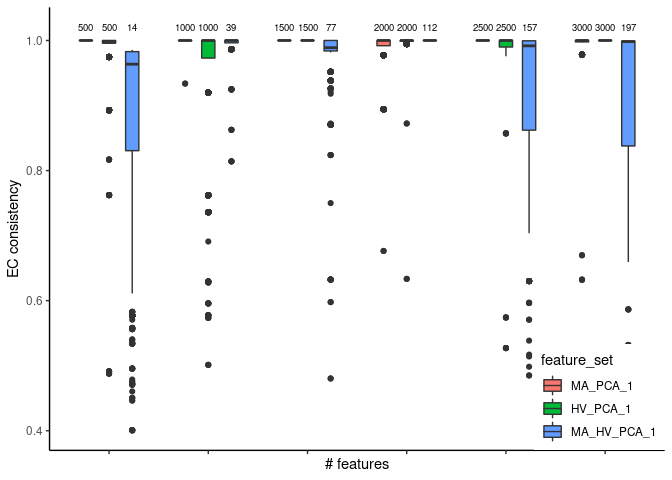
\includegraphics[width=0.8\linewidth]{images/ch3/3_feat_incremental.png}}
    \caption{\label{fig:ca-feat-inc} \textbf{Assessment of Feature stability, summarised as boxplots, obtained on 30 runs.} The colours indicates different feature sets, used for calculating the PCA: MA - most abundant genes (red); HV - highly variable genes (green); MA\_HV - intersection of MA and HV genes (blue). Above each boxplot we indicate the number of features within the subset. For this dataset, the MA and HV gene sets on 3000 genes are preferred due to their high consistency across the runs.}
\end{figure}

\subsubsection{Incremental similarity}
An important task in the data processing is identifying the noise. In single-cell analysis, this task translates into identifying the noisy genes, namely the features not only do not contribute to cluster identification, but also can perturb the output. This plot relates to this tasks and shows the distribution of the ECS between the partitions that are obtained using the same feature set, but with different sizes. The grouping is done in a similar fashion with the one from the previous plot. Our approach is to translate incremental dissimilarity as an indicator of not reaching the noise. The goal is to identify the transition from the signal to the noise zone.

Figure \ref{fig:ca-feat-comp} shows the Incremental similarity plot for the Cuomo data. As the title suggests, the comparison is done incrementally: first we compare the results obtained with 500 features with the ones when using 1000, then compare 1000 with 1500 and so on. It can be noticed that for MA\_HV the noise zone has not been reached, as the last blue boxplot suggests that adding the last genes has a signifcant impact upon the final clustering. As for the other two feature types, the high distribution of similarity in the last two groups of boxplots suggests that using more than 3000 genes would not lead to any information gain.

\begin{figure}[H]
    \centering
    \makebox[\textwidth][c]{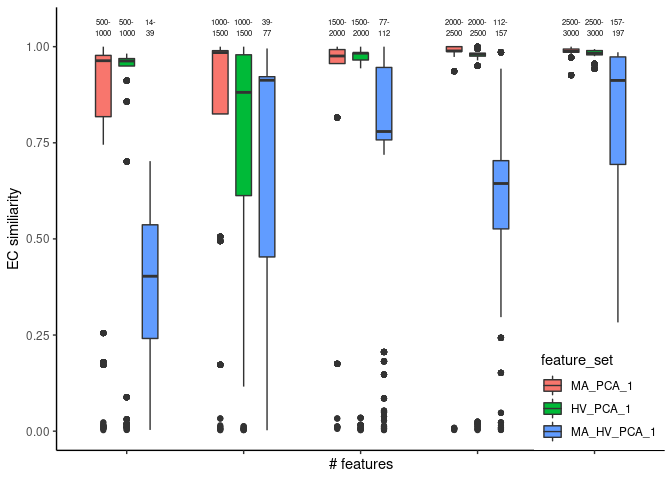
\includegraphics[width=0.8\linewidth]{images/ch3/3_feat_comparative.png}}
    \caption{\label{fig:ca-feat-comp}Clustering distribution with default parameters for Monocle (left) and Seurat (right). The title indicates the default random seed that is used.}
\end{figure}

\subsubsection{Distribution of clusters}
The last two plots provide information about the number of genes that should be used and the consistency of the feature set, but the consistency can have multiple causes. One factor that can influence the stability is the topology of the data. The following plot illustrates the cluster distribution for each subset of genes on the UMAP space.

An example of this plot can be seen in Figure \ref{fig:ca-feat-cluster}. Looking at the most abundant genes, we can notice that the high consistency is directly caused by the scattered distribution of the cells across multiple islands. HV and MA\_HV sets tend to produce more compact group of points, which might lead to a more relevant biological interpretation. Thus, using the stability assessment as well as the topology, the most suitable option should be the highly variable set having 2500-3000 genes.

\begin{figure}[H]
    \centering
    \makebox[\textwidth][c]{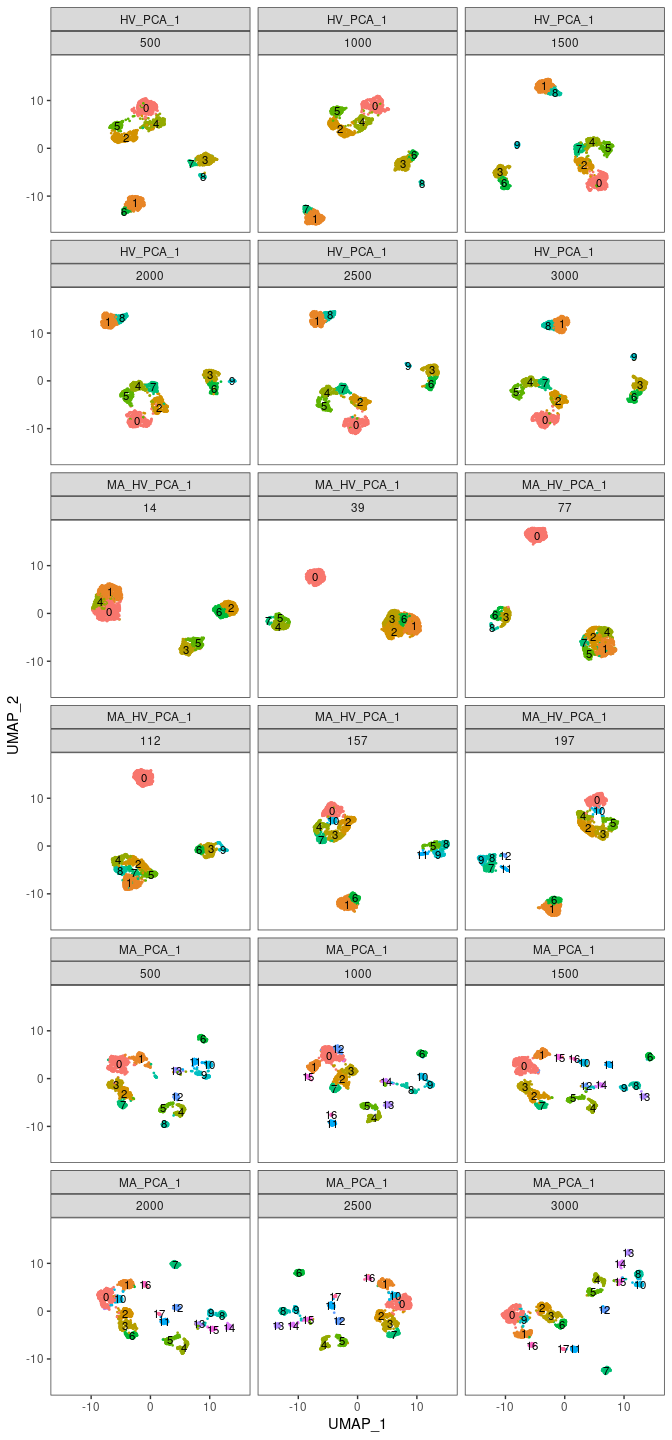
\includegraphics[width=0.6\linewidth]{images/ch3/3_feat_clusters_facet.png}}
    \caption{\label{fig:ca-feat-cluster}Clustering distribution with default parameters for Monocle (left) and Seurat (right). The title indicates the default random seed that is used.}
\end{figure}

\subsubsection{Stability areas}
This plot complements the previous one and displays the distribution of the ECC score on the UMAP topology, as it can be seen in Figure \ref{fig:ca-feat-stab}. This plot is taking advantage of the useful proprierty of the Element-Centric Similarity score and allows the user to identify the stable group of cells and the areas where the clustering in not consistent.

\begin{figure}[H]
    \centering
    \makebox[\textwidth][c]{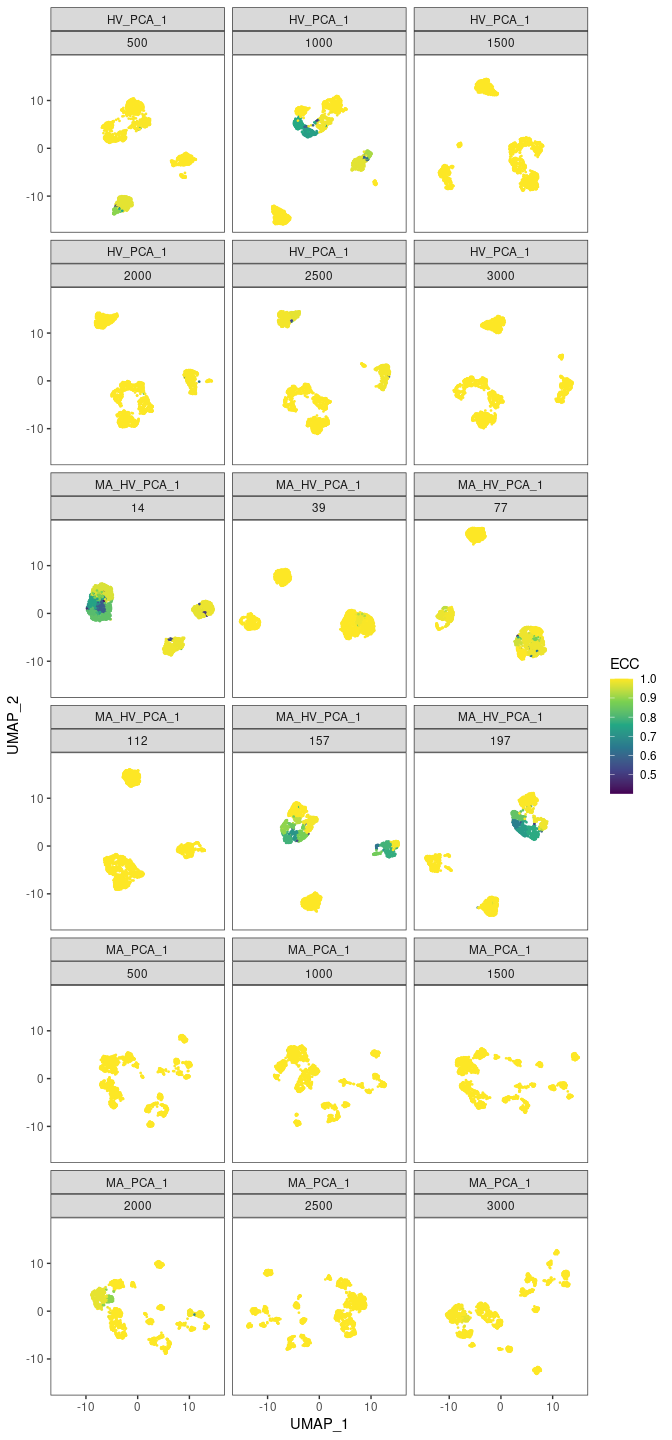
\includegraphics[width=0.6\linewidth]{images/ch3/3_feat_stab_facet.png}}
    \caption{\label{fig:ca-feat-stab}Clustering distribution with default parameters for Monocle (left) and Seurat (right). The title indicates the default random seed that is used.}
\end{figure}

\subsection{Assessing the graph construction}
Moving on the graph construction step, the most important parameters are the following:
\begin{itemize}
    \item base embedding: PCA or UMAP
    \item the number of neighbours: it is intuitive to say that using more neighbours would not damage or affect the clustering results; the purpose of including this parameter is that its values have an impact over the execution efficiency of the whole pipeline. Having more neighbours would lead to more calculations. Thus, our package allows the user to search for small values of the $k$ parameter that could be stable and relevant for the desired output.
    \item the graph type: unweighted (NN) or weighted (SNN)
\end{itemize}

Our package does not assess the change of the distance metric, as the \verb|RANN| package does not currently have support for changing this parameter.
For this step, ClustAssess can output three types of plots.

\subsubsection{Connected components target}
Since we are using community detection methods for graph clustering, it is unlikely (if not impossible) to obtain a cluster that contains two connected components. This type of merging (or moving a node to a cluster from another connected component) does not bring any improvement on the value of the quality function. One exception is related to the singleton clusters, which can be merged inside one single group or can be appended to the community in the closest proximity.

Therefore, the number of connected components acts like a lower bound for the possible number of clusters. The plot discussed in this section illustrates the impact that the number of nearest neighbours has on the number of connected components. The results are obtained by running the clustering pipeline multiple times while changing the seed. Thus, for each number of $k$, a boxplot distribution of the number of connected components will be displayed. PCA and UMAP can be used as base embedding. 

Figure \ref{fig:ca-conn-comp} shows how increasing the number of neighbours monotonically decreases the number of connected components, which is an expected behaviour, as more neighbours leads to more edges and to better connectivity. We notice how PCA requires only four number of nearest neighbour to reach a connected graph, while UMAP converges to a number of four. 

The utility of this plot resides in the ability to determine the appropriate number of neighbours that should be used to obtain at least a desired number of clusters. In our example, if we would want to get a number of five clusters when using UMAP as base embedding, the plot suggest that we should use at least 10 nearest neighbours.

\begin{figure}[H]
    \centering
    \makebox[\textwidth][c]{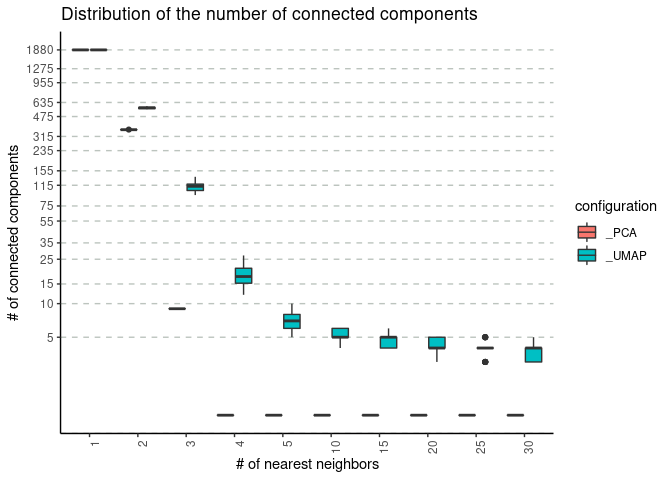
\includegraphics[width=0.6\linewidth]{images/ch3/3_conn_comp.png}}
    \caption{\label{fig:ca-conn-comp}Clustering distribution with default parameters for Monocle (left) and Seurat (right). The title indicates the default random seed that is used.}
\end{figure}

\subsubsection{Relationship between the number of clusters and number of neighbours}
The following type of plot graphically represents the relationships the number of neighbours and the actual number of clusters. Besides the graph embedding, the graph type can also be changed. The number of clusters is displayed as a boxplot distribution (see explanation at the previous plot). This plot can be used to infer the expected number of clusters on different configuration of these three parameters when the clustering algorithms is used with its default settings.

An example is provided in Figure \ref{fig:ca-nn-k}. We can notice the same decreasing tendency as in the connected components case when using more nearest neighbours. In our case, the graph type does not have a great impact over the number of clusters, but the base embedding does: PCA-based graphs are clustered in less communities.

\begin{figure}[H]
    \centering
    \makebox[\textwidth][c]{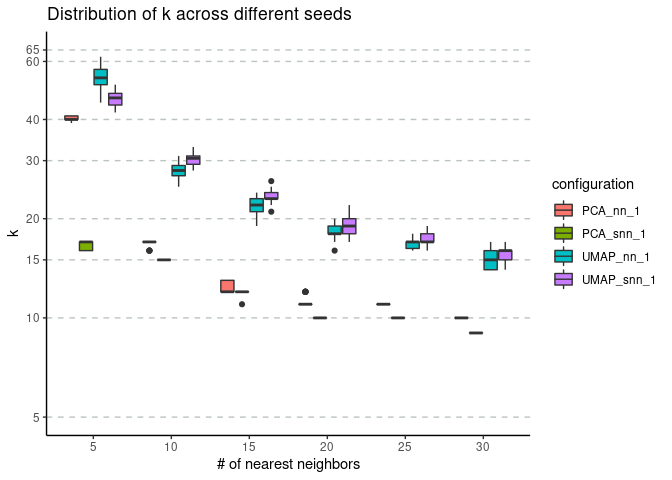
\includegraphics[width=0.6\linewidth]{images/ch3/3_nn_k.png}}
    \caption{\label{fig:ca-nn-k}Clustering distribution with default parameters for Monocle (left) and Seurat (right). The title indicates the default random seed that is used.}
\end{figure}

\subsubsection{Graph building stability}
This plot evaluates the stability of different configurations of the three parameters involved in the graph construction. Its use-case is to help the user choose the values that lead to robustness at changes of the random seed. Similarly to the Feature stability distribution plot, the stability is assessed using the ECC score. Its distribution is displayed using a boxplot distribution. The boxplots are grouped based on the different configurations.

For example, if Figure \ref{fig:ca-nn-ecc} we have four configurations as a result of combining the PCA and UMAP embedding with NN and SNN graph types. THere are more conclusions to be drawn from this plot:
\begin{itemize}
    \item given that UMAP is more reliant on the initial seed than the PCA, the results obtained from the latter are significantly more consistent.
    \item increasing the number of neighbours leads to the improvement of the stability.
    \item adding weights to the graph might lead to more consistent results.
\end{itemize}
\begin{figure}[H]
    \centering
    \makebox[\textwidth][c]{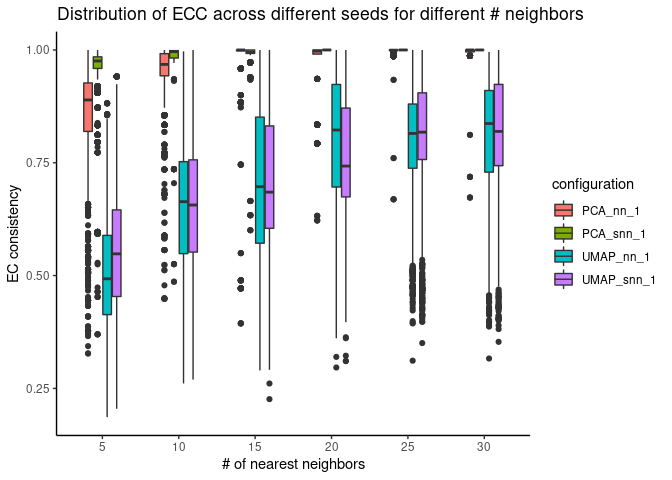
\includegraphics[width=0.6\linewidth]{images/ch3/3_nn_ecc.png}}
    \caption{\label{fig:ca-nn-ecc}Clustering distribution with default parameters for Monocle (left) and Seurat (right). The title indicates the default random seed that is used.}
\end{figure}

\subsection{Assessing the graph clustering}
Once the dimensionality reduction is performed and the graph is built, the remaining task is to assess the stability of the clustering. ClustAssess offers visual tools to evaluate the consistency of the community detection method, as well as of its most relevant parameter, the resolution.

\subsubsection{Clustering method stability}
ClustAssess uses Seurat for the implementation of the Phenograph pipeline, thus the available community detection methods are Louvain \cite{Blondel2008b}, Louvain with multi-level refinement \cite{Rotta2011}, SLM \cite{Waltman2013} and Leiden \cite{Traag2019a}. The following plot illustrates, for a given range for the resolution parameter, the distribution of the ECC. The procedure is slightly different from the previous steps: instead of taking all the partitions obtained after multiple runs with different seeds, we extract the number of clusters that appears the most frequent and we calculate the consistency of the clusterings having that number of groups. Above each boxplot the most common number of clusters will be displayed. This enables comparing the community detection methods not only by stability, but also by the number of clusters they will most probably output.

An example is provided in Figure \ref{fig:ca-clust-dif-boxplot} where the stability of the four clustering algorithms are assessed on the Cuomo dataset. Leiden (with red colour) followed by Louvain (green) are noticeably less consistent than the other two methods, thus the conclusion the user could draw from this plot is that Louvain refined or SLM are more suitable choices to reach robust results.

\begin{figure}[H]
    \centering
    \makebox[\textwidth][c]{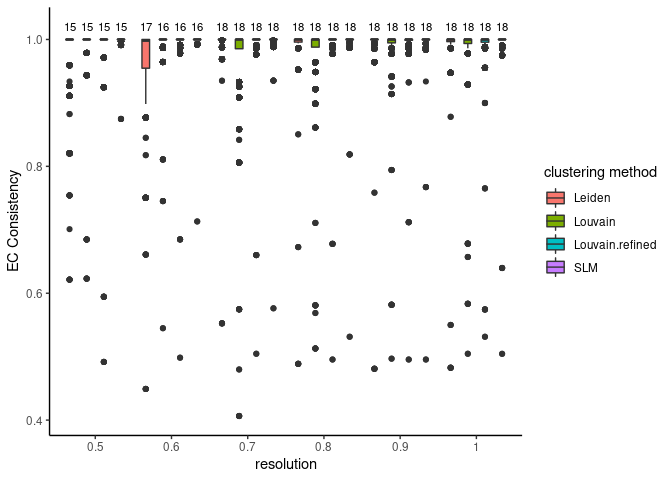
\includegraphics[width=0.6\linewidth]{images/ch3/3_clust_dif_boxplot.png}}
    \caption{\label{fig:ca-clust-dif-boxplot}Clustering distribution with default parameters for Monocle (left) and Seurat (right). The title indicates the default random seed that is used.}
\end{figure}

\subsubsection{Areas of clustering consistency}
To reinforce the previous plot, ClustAssess also offers support for visualising the distribution of the ECC score on an UMAP representation. The plot is faceted, so each column will be associated with one clustering method and each row with a resolution value. This plot can serve as a tool to identify the areas that are unstable, as well to assess whether the instability occurs at all algorithms in the same areas or not. We note that, in this case, the ECC will be calculated across all partitions that are obtained without filtering by a specific number of clusters.

An example is provided in Figure \ref{fig:ca-clust-dif-facet}. It's noticeable how Leiden's behaviour is different from the other three: the main area of instability is located in the upper island. Louvain also has more incosistent areas when resolution is greater than 0.6. SLM and Louvain refined seem to behave similarly with few exceptions: for resolution 0.5 or 0.7, where the latter has an additional unstable region. The conclusion the user could draw is that SLM has the most robust behaviour, as there are a few number of unstable areas; in addition to that, those areas are unstable in the other algorithms as well.

\begin{figure}[H]
    \centering
    \makebox[\textwidth][c]{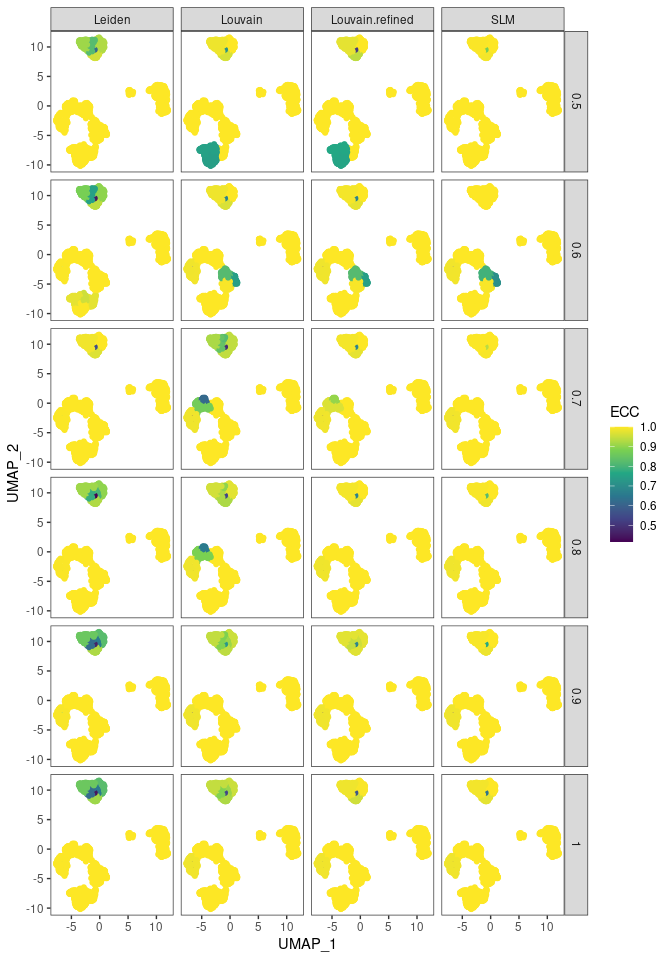
\includegraphics[width=0.6\linewidth]{images/ch3/3_clust_dif_facet.png}}
    \caption{\label{fig:ca-clust-dif-facet}Clustering distribution with default parameters for Monocle (left) and Seurat (right). The title indicates the default random seed that is used.}
\end{figure}

\subsubsection{Resolution - number of cluster correspondence}
One of the limitation of the community detection method is that there is no direct way to specify the number of desired clusters, like in other clustering algorithms such as k-means. The number of clusters is directly affected by the resolution parameter, but the relationship between these two values is dependent on the graph's structure.

The following plot is meant to illustrate this correspondence between the two parameters. On the X-axis different resolution values provided by the user are displayed, and the Y-axis contains the number of clusters. The correspondence is displayed using a scatter plot. One immediate use-case for it is to identify the suitable resolution values to obtain a desired number of clusters. 

This plot also offers additional information regarding the stability of the resolution parameter - number of clusters pair. Firstly, the point size is varying based on the frequency of the most common partition obtained when fixing the resolution and the number of clusters. Thus, large points are a measure for high stability, as they indicate that even if the seed is changed, the same partition will be obtained.

\begin{figure}[H]
    \centering
    \makebox[\textwidth][c]{
        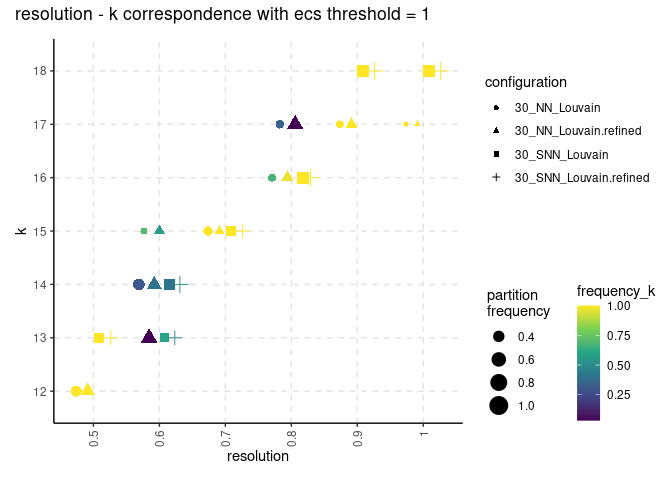
\includegraphics[width=0.5\linewidth]{images/ch3/3_1_kres_freq.png}
        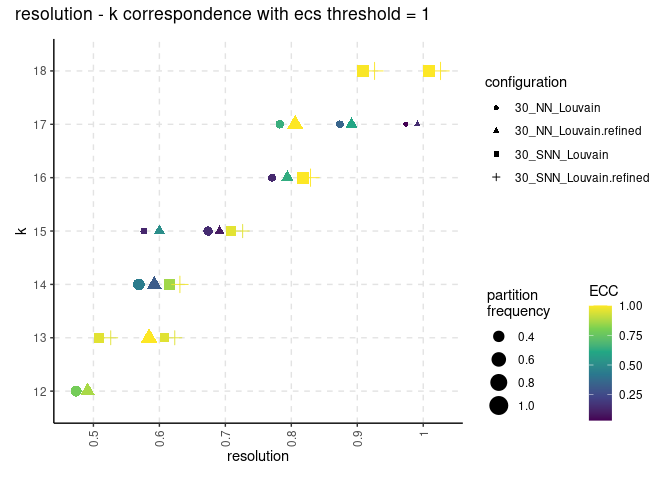
\includegraphics[width=0.5\linewidth]{images/ch3/3_1_kres_ECC.png}}
    \caption{\label{fig:ca-1-kres}Clustering distribution with default parameters for Monocle (left) and Seurat (right). The title indicates the default random seed that is used.}
\end{figure}

\subsubsection{Stability of the number of clusters}
As can be observed from Figure \ref{fig:ca-1-kres}, multiple values of the resolution parameter can lead to partitions with the same number of clusters. Therefore, the task evolves from identifying stable pairs of resolution - number of clusters values to finding the number of clusters that is stable for any resolution value.

This plot removes the resolution dependency, so the partitions with the same number of communities are kept into the same list, compared to the previous approach, where they were separated by the extra-layer added by resolution. The scatter plot approach is kept, but on the X-axis the number of clusters is displayed, whereas the Y-axis contains the number of unique partitions with the same number of clusters. This is the first information that could be used in order to infer the stability: if there are many unique partitions that could be obtained, it is probable that the number of clusters is unstable.

The colour gradient provides additional information regarding the stability. Currently, there are two options for the information transmitted through the colour gradient: either the frequency of the most common partition, or the ECC of the list of partitions with the same number of clusters. Lighter shades (close to yellow) indicate high robustness, while low shades (close to dark blue) define instability. Both the colour gradient and the number of unique partitions can be used in order to assess the consistency of the number of clusters.

There could be situations when a number of clusters is present in only one partition that appears once. Although it could be considered stable, the data is insufficient to draw a conclusion. To verify the reliability of the previously-drawn conclusions, the point size is used to show the frequency of the partitions having a specific number of clusters. Thus, large points are indicator that the stability inference is made on a sufficient sample of partitions and can be trusted.

Similarly to the previous plot, the shape of points indicate different configurations where the varying parameters are the number of nearest neighbour, the graph type and the community detection algorithm.

An example is presented in Figure \ref{fig:ca-1-knpart}. The complexity of the plot allows to make multiple observations, such as the instability of the 17 as the number of clusters for "30\_NN\_Louvain" and "30\_N\_Louvain.refined". Also, we can notice that it is not redundant to use analyze both cases when the colour gradient represents the frequency of the most common partition (left panel) or the ECC of the list of partitions (right panel). There are cases, as the one when the number of clusters is 15, when the frequency is not convincing, but the high consistency provides the additional information that the other partitions are not significantly different from the most frequent one. We can remark the importance of the point size for 13 number of clusters with "30\_NN\_Louvain.refined" configuration: the stability is ranked high by both indicators, but the size of the point indicates that the sample used to calculate the stability is too small to be trusted. Two suitable choices that can be immediatly spotted are 16 and 18, where there is high stability, a small number of different partitions and a reasonable sample size.

\begin{figure}[H]
    \centering
    \makebox[\textwidth][c]{
        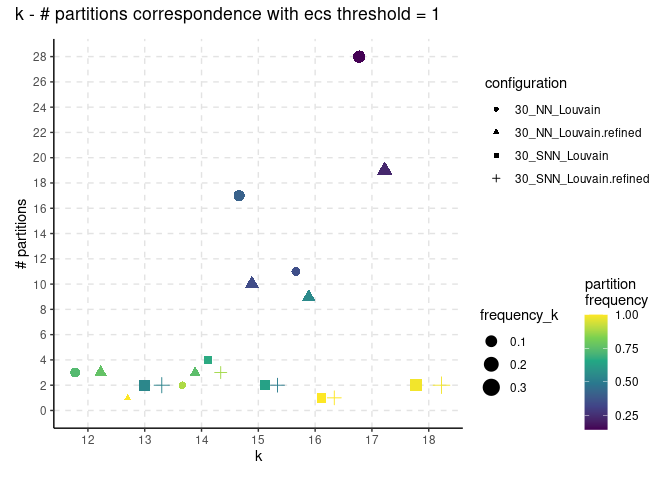
\includegraphics[width=0.5\linewidth]{images/ch3/3_1_knpart_freq.png}
        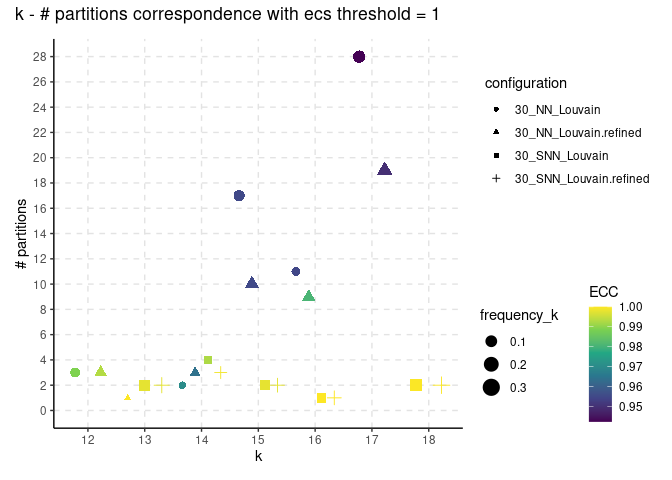
\includegraphics[width=0.5\linewidth]{images/ch3/3_1_knpart_ECC.png}}
    \caption{\label{fig:ca-1-knpart}Clustering distribution with default parameters for Monocle (left) and Seurat (right). The title indicates the default random seed that is used.}
\end{figure}

%\begin{figure}[H]
%    \centering
%    \makebox[\textwidth][c]{
%        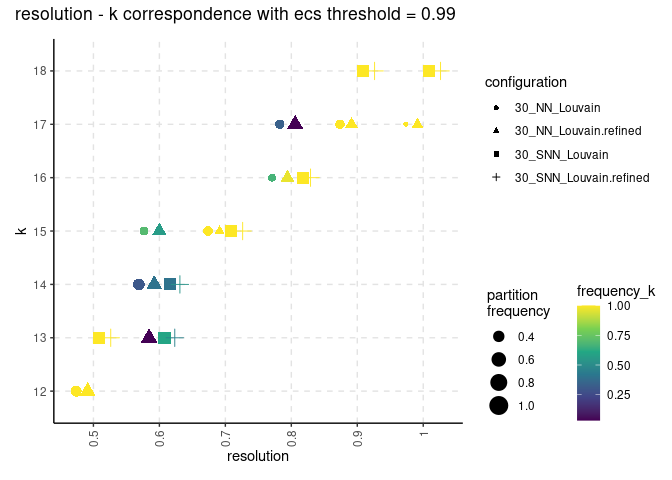
\includegraphics[width=0.5\linewidth]{images/ch3/3_99_kres_freq.png}
%        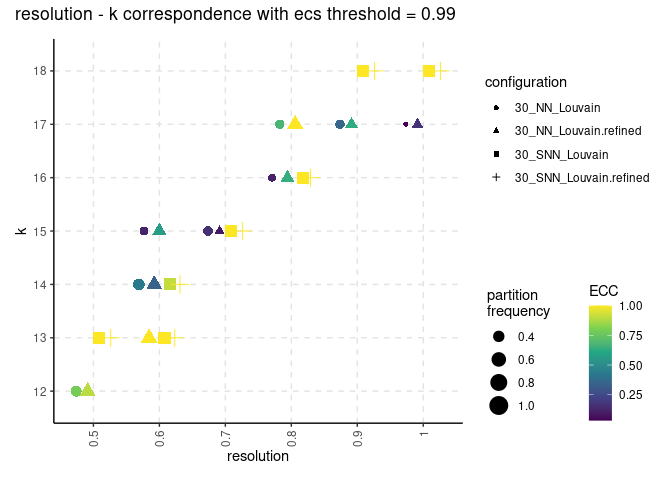
\includegraphics[width=0.5\linewidth]{images/ch3/3_99_kres_ECC.png}
%    }
%    \caption{\label{fig:ca-99-kres}Clustering distribution with default parameters for Monocle (left) and Seurat (right). The title indicates the default random seed that is used.}
%\end{figure}
%\begin{figure}[H]
%    \centering
%    \makebox[\textwidth][c]{
%        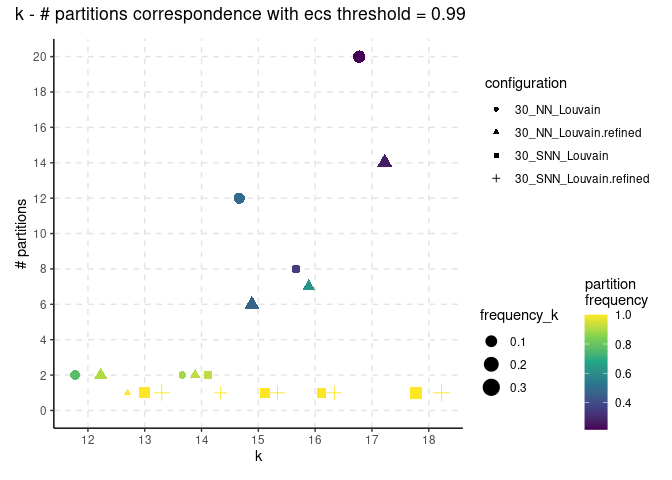
\includegraphics[width=0.5\linewidth]{images/ch3/3_99_knpart_freq.png}
%        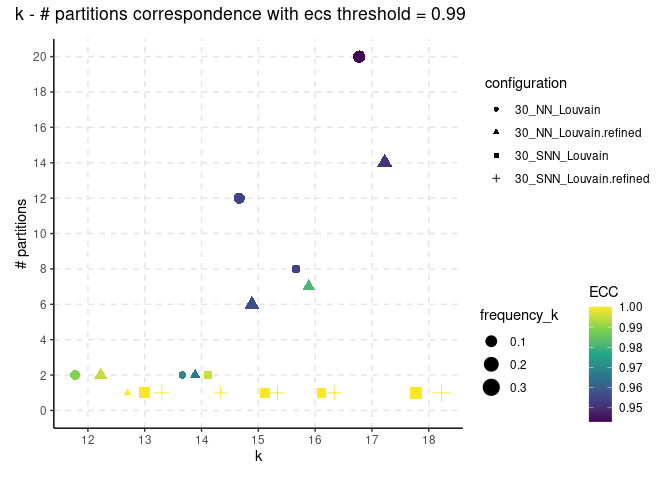
\includegraphics[width=0.5\linewidth]{images/ch3/3_99_knpart_ECC.png}}
%    \caption{\label{fig:ca-99-knpart}Clustering distribution with default parameters for Monocle (left) and Seurat (right). The title indicates the default random seed that is used.}
%\end{figure}
